%************************************************************************************************************
\section{Computer Simulation and Safety Analysis of Nuclear Power Plant}\label{sec:intro_computer_simulation}
%************************************************************************************************************

The ubiquity of computer simulation applications in many fields of science and engineering results in an even more pervasive definitions of the term \textit{scientific computer simulation} itself 
and other associated terms such as \textit{model} and \textit{simulation}.
\marginpar{scientific computer simulation}
Though most of the definitions in the literature are not necessarily in contradiction to each other, 
to avoid confusion, this thesis adopts a recent definition proposed by Kaizer et al.\cite{Kaizer2015} quoted below,

\begin{quote}
	Scientific Computer Simulation is the imitation of a behavior of a system, entity, phenomenon, or process in the physical universe 
	using limited mathematical concepts, symbols, and relations through the exercise or use of scientific computer model.
\end{quote}

There are three main points highlighted in this definition.
\marginpar{model, simulation, and computer simulation}
First, this definition accentuates the difference between a \emph{model} and its \emph{simulation}.
Specifically, the former deals with the notion of representation, while the latter deals with the notion of imitation of a behavior.
Secondly, what makes a model scientific is that it treats physical phenomena or the behavior of a real world system as its subject.
Thirdly and finally, the modifier \emph{computer} in the definition makes it explicit that digital computer is used to solve whatever mathematical models serve as the representation.
This is usually the case for mathematical models that cannot be solved analytically.
Though this limitation what makes a solution of the model possible in the first place, 
it also affects the solution and its possible interpretation and thus many computational-related aspects also need to be comprehensively considered.

Beven \cite{Beven2009} articulates this distinction into three levels of model: perceptual model (i.e., theoretical description of some physical phenomena), formal model (i.e., the mathematical description of it), and procedural model  (i.e., computer implementation of the formal model). For many physical system modeling applications, only the procedural model is able to make a quantitative prediction of the system. These distinctions are useful in acknowledging the level of approximation involved in moving from perceptual to procedural model.

Granted, a simplicistic model cannot be expected to imitate all the important features of a complex physical phenomenon.
And yet, there is a tendency of developing and applying overly complex model, with numerous parameters and multiple non-linear relationships, for computer simulation.
This tendency has invited many critics over the year (citation needed).
In nuclear science and engineering, for instance, Zuber \cite{Zuber2001} and Wullf \cite{Wulff2007} have long critized the development and the use of multi-fluid model for thermal-hydraulics simulation as high in complexity and in maintenance cost, but low in fidelity and its usefulness.

The goal of computer simulation, complex or otherwise, is to provide prediction.
The main characteristic (and source of criticism) of using multi-parameter complex model for simulation is that the the relationship between numerous inputs and outputs becomes increasingly opaque.
The impact of changing one parameter alone, or especially together, on the prediction is hard to disentangle or intuit.
Furthermore, as appropriate values of inputs might not be fully known, they are often given simply over range of interest containing different possible permissible values.
It is thus seldom the case that one single simulation is sufficient to provide a reliable answer according to hardly any objective of computer simulation.
As analytical solution

\gls[hyper=false]{trace}

%---------------------------------------------------------------------------
\subsection{Thermal-Hydraulics System Codes}\label{sub:intro_th_system_code}
%---------------------------------------------------------------------------

% Introductory Paragraph
During the early days of reactor safety analysis, prediction using computer model of \gls[hyper=false]{npp} behavior during transient, off-normal or accident conditions, was approached with high-degree of conservatism.
Conservatism called for the most penalizing modeling assumptions to ensure conservative results, which is far below their regulatory limits.
This approach, though less realistic, was justified by limited modeling capabilities as well as limited knowledge of the physical process involved during those transients.
However, it was later found that there are conditions where conservative assumptions do not necessarily lead to conservative (or even physical) predictions.

% An Illustration
As an example of this contradiction, consider the following situation in the analysis of \gls[hyper=false]{loca} as described in \cite{IAEA2009}.
Assuming less interfacial shear between liquid and gas phase of the coolant (water) reducing mist flow during \gls[hyper=false]{loca} is conservative in the sense that less heat will be transferred to the coolant flow in the upper region of the core.
This, in turn, penalizes the fuel temperature prediction.
But this assumption also implies that the time to refill the core is shorter as there will be more liquid retained in the reactor cooling system.
Furthermore, with less shear, there is less resistance in injecting emergency coolant into the core (condition known as the counter-current flow limitation).
Both of these are clearly non-conservative and contradicting the initial conservative assumption.

% Best-estimate Analysis
Therefore, a more accurate prediction of two-phase flow transient behavior was deemed necessary for the safety analysis of nuclear power plant under accident conditions.
As opposed to the conservative analysis, the term for this approach was coined \emph{best-estimate} analysis.
Such an analysis calls for more physically sound thermal-hydraulics models with more realistic modeling assumptions which at the same time are also backed by experimental data obtained from numerous experimental programs conducted in Separate and Integral Effect Test Facilities.
With the idea of having more realistic prediction in mind, a best-estimate \gls[hyper=false]{th} system code was developed.
The code is designed to be a comprehensive tool capable of simulating realistically wide range of transients foreseen in \gls[hyper=false]{npp} operation.
It was developed using the current best understanding of flow processes expected to happen during the transients.

% Thermal-Hydraulics System Code
The typical structure of a system code is illustrated in Fig.~\ref{fig:ch1_th_system_code}.
As can be seen, system code constitutes of several building blocks that can be used to model and simulate wide range of system and conditions.
The core of system code is a set of balance equations describing the dynamics of the state variables of the fluid.
To close the system (i.e., to have the same number of equations as the number of unknowns), it has to be complemented by two additional set of constitutive equations.
The first is the equation of state describing the thermodynamic relation between state variables of a given fluid.
The second is the closure relationships describing the interaction between phases and each phase to the boundary wall in terms of mass, momentum, and energy. 
\begin{figure}[bth]	
	\centering
	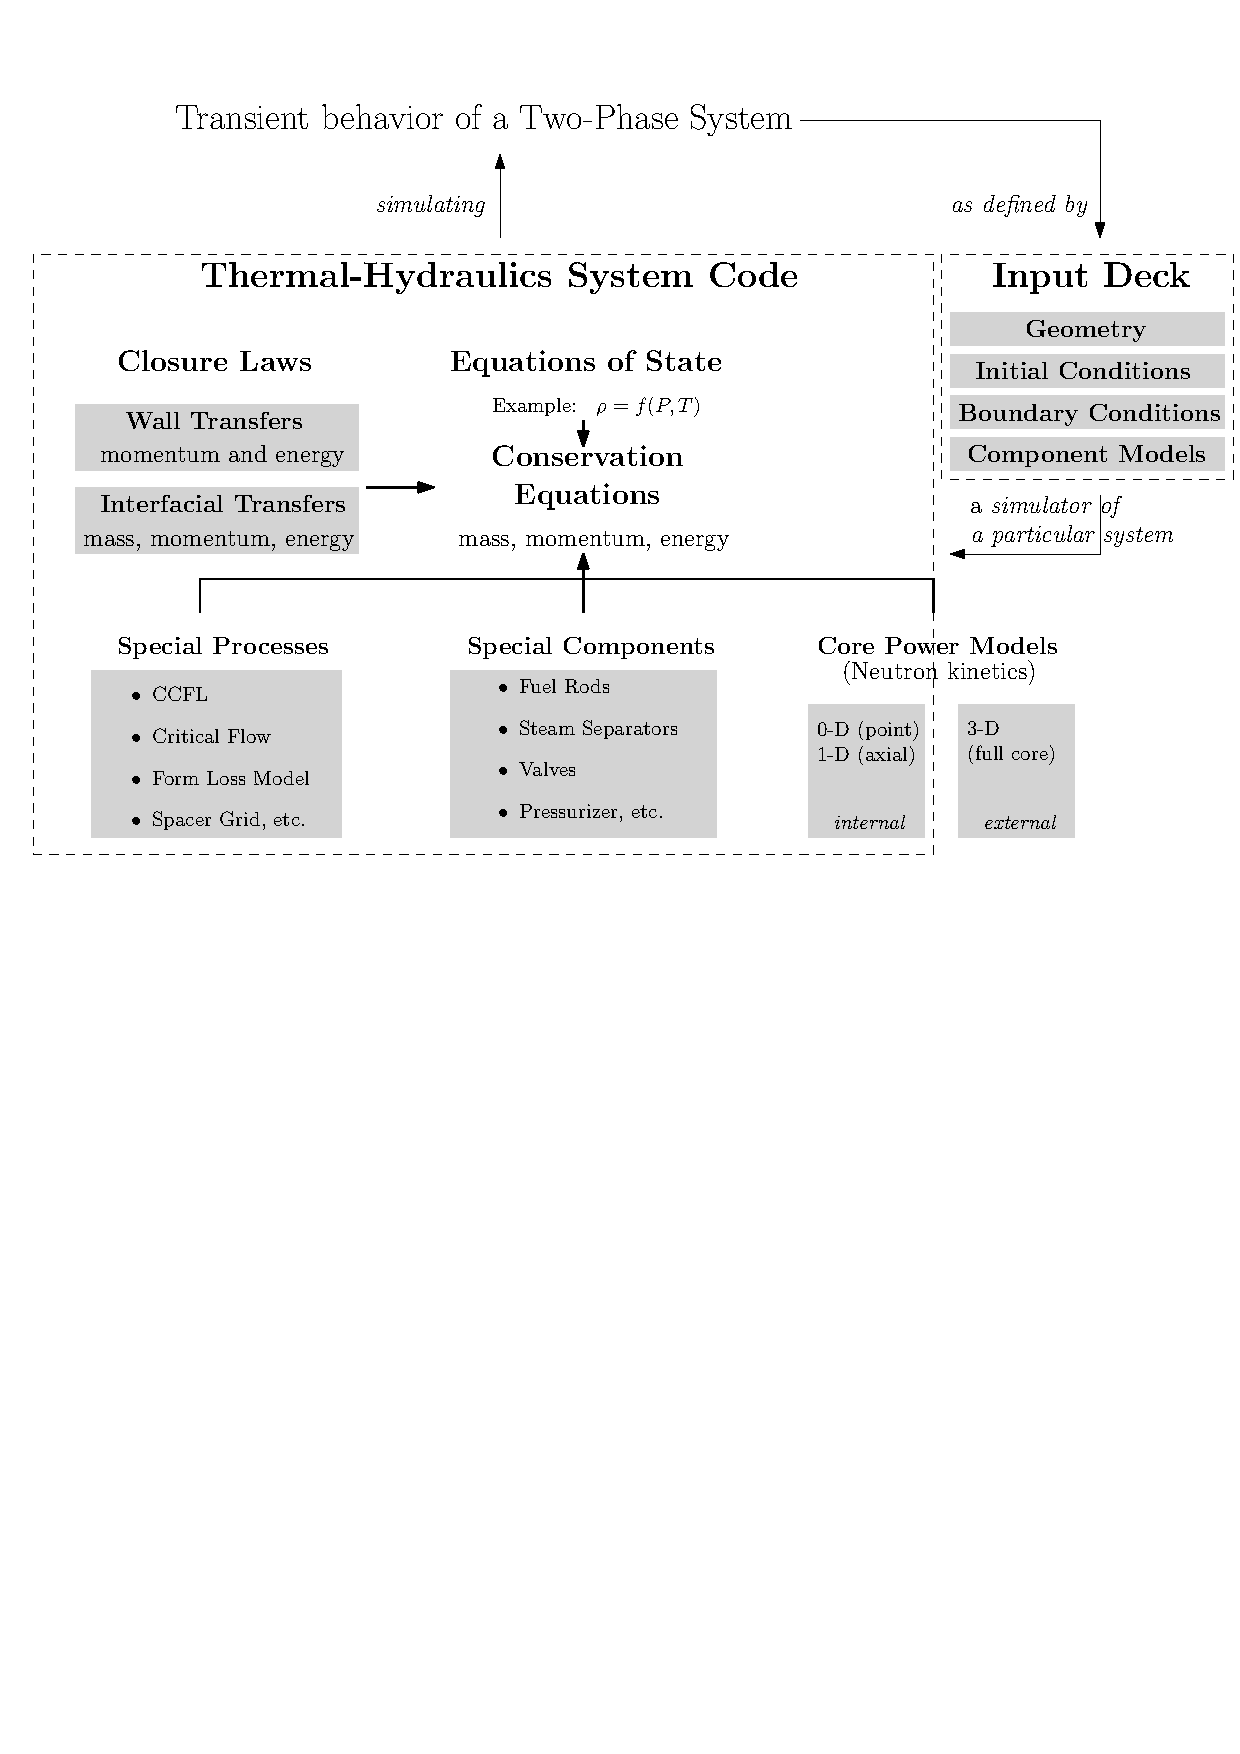
\includegraphics[width=\textwidth]{../figures/chapter1/figures/th_system_code}
	\caption[Generic structure of a thermal-hydraulics (TH) system code]{Generic structure of a \glsfirst[hyper=false]{th} system code. The code and the specific system defined by the input deck define a \emph{simulator} of that system.}
	\label{fig:ch1_th_system_code}
\end{figure}

% Two-fluid Model

% Validity of Two-fluid Model

% Closure Laws
